\begin{frame}
    \frametitle{Baseline understanding - Mesh convergence}
    \begin{itemize}
        \item Balance between precision and computational time
    \end{itemize}
    \begin{table}[scale=0.4]
    \begin{tabular}{ccc}
        \textbf{Mesh size [\si{\milli\metre}]} & \textbf{Total CPU time [\si{\second}]} & \textbf{Displacement [\si{\nano\metre}]}\\ \hline
        10   & 14  & 68\\
        5    & 17  & 67\\
        \alt<2>{\color{red}2.5}{2.5}  & \alt<2>{\color{red} 47}{47}  & \alt<2>{\color{red} 63}{63}\\
        1.25 & 303 & 62
    \end{tabular}
    \end{table}
    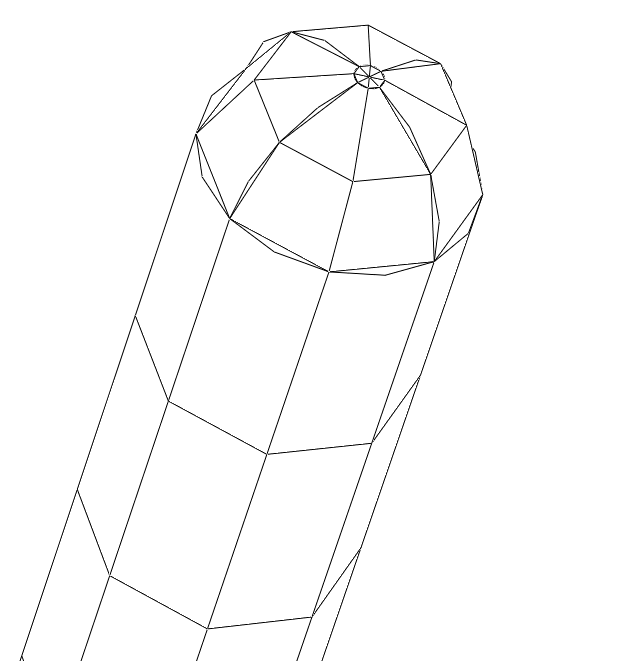
\includegraphics[width=0.24\textwidth]{../Modelling/Mesh convergence/0.01-tip.png}
    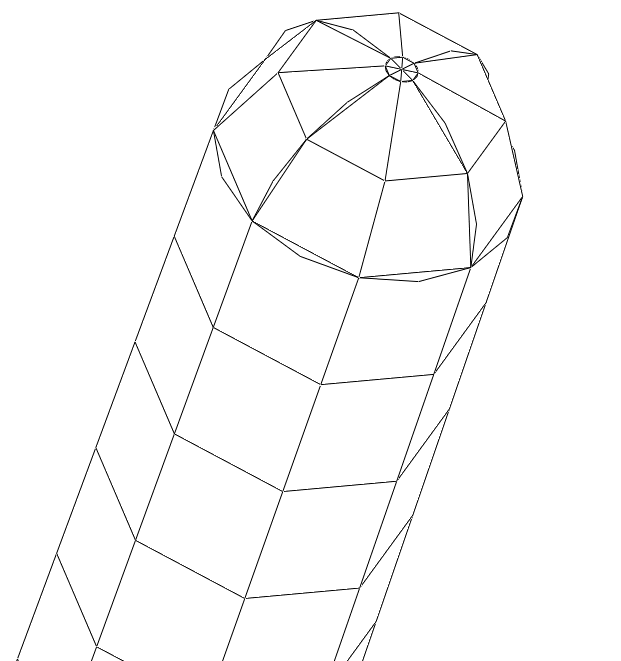
\includegraphics[width=0.24\textwidth]{../Modelling/Mesh convergence/0.005-tip.png}
    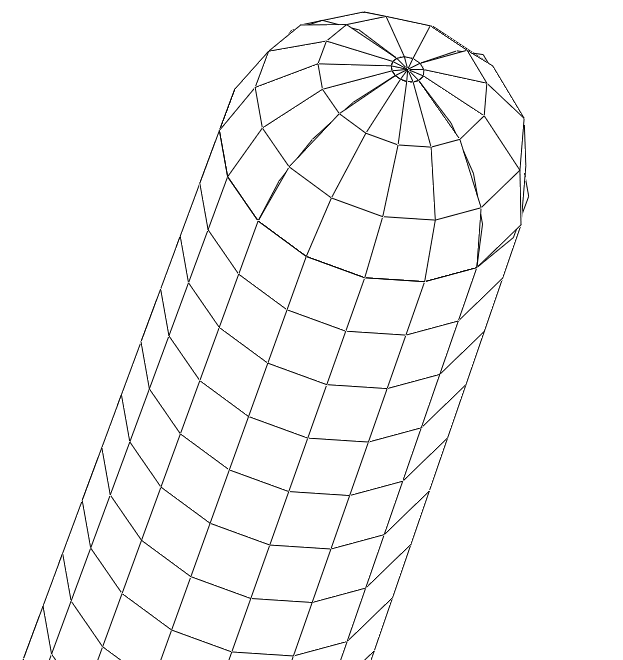
\includegraphics[width=0.24\textwidth]{../Modelling/Mesh convergence/0.0025-tip.png}
    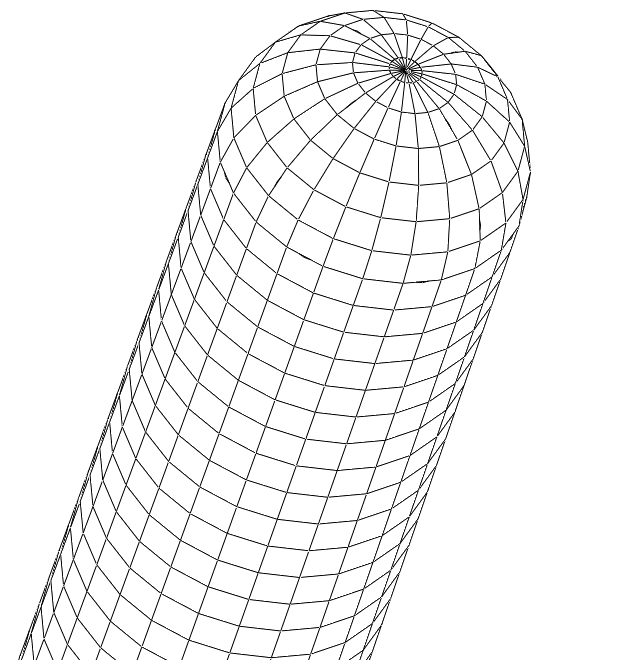
\includegraphics[width=0.24\textwidth]{../Modelling/Mesh convergence/0.00125-tip.png}
\end{frame}

\begin{frame}
    \frametitle{Baseline understanding - Linearity}
    \begin{itemize}
        \item Verify expectations of linear behaviour
    \end{itemize}

\end{frame}